\documentclass{article}

\usepackage{iclr2026_conference,times}
\input{math_commands.tex}
\usepackage{hyperref}
\usepackage{url}
\usepackage{graphicx}
\usepackage{booktabs}
\usepackage{amsmath}
\usepackage{amssymb}
\usepackage{amsthm}

\emergencystretch=3em

\title{Tool Use Contact Grammar: Falsifiable Contact-Role Productions for Robot Tool Use}

\author{Anonymous Authors}

\newtheorem{theorem}{Theorem}
\newtheorem{proposition}{Proposition}
\newtheorem{definition}{Definition}
\newtheorem{assumption}{Assumption}
\newcommand{\CG}{\textsc{Contact Grammar}}
\newcommand{\Cstate}{\mathcal{S}}
\newcommand{\Rules}{\mathcal{R}}
\newcommand{\Trace}{\tau}

\begin{document}
\maketitle

\begin{abstract}
Robot tool use is often represented as an affordance label, a task-conditioned grasp, a contact mode sequence, or a language-conditioned skill. These views can hide a brittle assumption: that the order and role of contacts among hand, tool, target, and environment can be recovered later or treated as a low-level control detail. We propose a contact grammar whose production rules create, transform, and test typed contact-role predicates. A tool-use plan is an ordered derivation, and a failure is a falsified production precondition. The contribution is representational and diagnostic rather than a new robot controller: contact-role productions expose which physical relation is required, which observation supports it, and which counterfactual precondition would create a false positive. We give a finite-state soundness/completeness statement for calibrated productions and evaluate the mechanism in an expanded finite contact world with 15 task families, 14 morphology predicates, five operating profiles, production mutations, predicate-noise stresses, grammar-library incompleteness, role-granularity ablations, and adversarial counterexamples. In the baseline full-scale contact world, the fine contact grammar reaches F1 1.000 with false-positive rate 0.000. Static affordances reach F1 0.633 with false-positive rate 0.473, unordered contacts reach F1 0.702 with false-positive rate 0.347, and a local contact-bigram model reaches F1 0.769 with false-positive rate 0.246. Predicate noise exposes the main boundary: at 10\% independent symbolic-observation noise, direct grammar F1 falls to 0.861, while an idealized targeted-probe fallback restores F1 1.000 at mean 3.17 probes. The evidence is deliberately scoped to a symbolic simulator. It supports the claim that ordered, typed contact-role productions are a sharper hypothesis class for tool use than static affordances or unordered contacts; it does not claim real-robot deployment, learned perception, or continuous contact stability.
\end{abstract}

\section{Introduction}

Tool use is a contact story. A robot does not merely choose a hammer, hook, wedge, brush, scoop, clamp, or rod. It grips one part, brings another part to a target from a particular side, sometimes braces on the environment, and then transmits force through a mechanically meaningful chain. A hook touching the front of an object and a hook seated behind it have the same object pair but different mechanical meaning. A wedge under a lid without an environmental brace is not a pry. A flat edge touching debris after a poor grasp may be present but not force-transmitting. A compliant pad is helpful for wiping but not for levering a heavy box.

Many robot interfaces flatten this structure. Affordance methods expose object regions, action labels, or action possibilities \citep{gibson1979ecological,yamanobe2017affordance,ardon2021affordance}. Task-oriented grasping connects grasp and downstream action \citep{kokic2017affordance,fang2018tog}, but often leaves the full contact trace implicit. Contact-rich planning has deep mechanics \citep{mason1986pushing,erdmann1988sensorless,lynch1996stable,graesdal2024convex}, while task-and-motion planning uses symbolic skeletons and continuous checks \citep{kaelbling2011tamp,toussaint2015logic,garrett2020pddlstream}. Robot foundation and language-conditioned systems scale action selection \citep{ahn2022saycan,brohan2022rt1,brohan2023rt2,liang2023code,huang2023voxposer}, but their plan interfaces can still skip explicit physical contact preconditions.

This paper studies a narrower hypothesis: for robot tool use, the reusable unit should be an ordered, typed contact production. A production such as \textsc{SeatHookBehind} has typed preconditions over tool morphology, hand-tool grasp, target side access, and current contact state; its effect adds a contact predicate that later productions consume. A production such as \textsc{RotateAboutBrace} requires a wedge contact and an environment brace before rotation. The grammar does not replace continuous control. It supplies a symbolic contact trace that says what the controller is supposed to make true and what would falsify the plan.

The paper's claim is not that affordances are useless, that contact mechanics are solved, or that language planners cannot help. The claim is that static labels and unordered contact sets conflate traces that differ in physical validity. Contact role and order are not mere bookkeeping; they are part of the hypothesis class. A representation that exposes them can reject invalid traces that a feature-only system accepts, and it can fail in interpretable ways when predicates are missing or noisy.

The contributions are:
\begin{itemize}
    \item We define a contact grammar for tool use as a finite set of typed production rules over hand-tool-target-environment contact predicates.
    \item We give a conditional finite-state guarantee: calibrated productions are sound and complete for traces in the grammar closure up to a bounded depth.
    \item We introduce a falsification protocol: remove or coarsen individual preconditions and measure the resulting false-positive or false-negative signature.
    \item We release a full-scale symbolic contact-world evaluation with expanded tasks, tools, baselines, noise, mutations, library incompleteness, granularity ablations, cost summaries, and counterexamples.
\end{itemize}

The evidence is intentionally scoped. The production library is hand-designed. Predicate perception is either exact or synthetically corrupted. Continuous stability, friction cones, slip, deformation, tactile estimation, and controller synthesis are coarse symbolic gates. The goal is to make the representational claim precise before claiming robot deployment.

\section{Related Work and Novelty Boundary}

\paragraph{Affordances and tool use.}
Affordances originate as action possibilities between agent and environment \citep{gibson1979ecological}. Robotics has used affordance representations for manipulation, grasping, and tool use \citep{stoytchev2005tool,sinapov2007tool,yamanobe2017affordance,ardon2021affordance}. Tool-use work has learned behavior-grounded categories, task-oriented grasps, and morphology-conditioned actions \citep{fang2018tog,shao2020tools,qinsurvey2023,yang2024granularity}. These works pressure any claim that ``tools need action-conditioned representations'' is new. Our boundary is more specific: a tool-use plan should be an ordered derivation over typed contact roles, and each production should expose falsifiable preconditions.

\paragraph{Task-oriented grasping.}
Task-oriented grasping correctly argues that the right grasp depends on the downstream task \citep{kokic2017affordance,fang2018tog}. \CG{} is complementary. A production such as \textsc{GraspHandle} can encode the hand-tool role needed for later contact productions, but the grammar also models target and environment contacts after grasping. The representation is not just where to grasp; it is how contacts are sequenced and consumed.

\paragraph{Contact-rich manipulation and mechanics.}
Classical manipulation mechanics model pushing, sensorless manipulation, stable contact, and dynamic behavior composition \citep{mason1986pushing,erdmann1988sensorless,lynch1996stable,burridge1999sequential}. Modern contact-rich planners and relaxations reason through hybrid contact choices \citep{toussaint2015logic,graesdal2024convex}. \CG{} does not replace those methods. It sits above them as a compact symbolic trace language: it can prune impossible contact stories and diagnose which role or precondition must be realized by the continuous layer.

\paragraph{Task-and-motion planning.}
TAMP systems interleave symbolic action choices with geometric and continuous feasibility checks \citep{kaelbling2011tamp,toussaint2015logic,garrett2020pddlstream}. \CG{} can be seen as a domain-specific symbolic layer for tool-use contact. The distinction is the production vocabulary: rules are organized around hand-tool-target-environment roles and their ordered effects, not only object predicates or stream calls.

\paragraph{Language and foundation-model planners.}
Language-conditioned robot systems can produce broad plans or spatial action hints \citep{ahn2022saycan,brohan2022rt1,brohan2023rt2,liang2023code,huang2023voxposer,wi2023calamari}. These systems make ``use language to plan'' a weak novelty claim. Here language may specify the goal, but the contact grammar rejects or accepts a plan through typed physical preconditions. The grammar is the audit layer that says whether ``use the hook to pull the ring'' has the right contact trace.

\paragraph{Novelty boundary.}
The novelty is not ``contact matters'' or ``affordances matter.'' The novelty is to treat contact-role productions as the planner-facing unit of tool-use composition and falsification. The experiments are designed around this boundary: baselines have access to features, unordered contacts, local contact pairs, memory, or task priors, but not the full ordered role derivation.

\section{Problem Setup}

Let $H$, $U$, $O$, and $E$ denote hand, tool, target object, and environment. A symbolic contact state $s\in\Cstate$ is a finite set of typed predicates such as
\[
    \texttt{hand:tool\_handle},\quad
    \texttt{tool:target\_behind},\quad
    \texttt{tool:environment\_brace}.
\]
Tool morphology is represented by predicates and attributes: hook, wedge, flat edge, narrow tip, long shaft, soft pad, high friction, clamp jaw, length, stiffness, compliance, friction, and handle offset. Task predicates specify target side, required features, force class, fragility, slippery surface, and whether an environmental brace is needed.

\begin{definition}[Contact production]
A contact production $r\in\Rules$ is a tuple $(\tau,P,A,D)$ with type signature $\tau$, preconditions $P$, additive effects $A$, and deleted or invalidated predicates $D$. It is applicable in state $s$ when all preconditions are satisfied. Applying it yields $(s\setminus D)\cup A$.
\end{definition}

\begin{definition}[Contact derivation]
A contact derivation is an ordered sequence $(r_1,\ldots,r_T)$ of applicable productions. The derivation is valid for a task if it reaches a state satisfying the task's terminal contact-role predicate and all mechanical gates remain satisfied.
\end{definition}

Examples include:
\begin{itemize}
    \item \textsc{GraspHandle}: creates a hand-tool role required before any tool-target production.
    \item \textsc{SeatHookBehind}: requires a hook-like feature, side access, and a previous grasp; creates a behind-contact predicate.
    \item \textsc{InsertWedgeUnder}: requires wedge or thin-lip morphology and target-side access; creates an under-contact predicate.
    \item \textsc{BraceOnRim}: requires environment support; creates a tool-environment brace predicate.
    \item \textsc{RotateAboutBrace}: consumes wedge-under and brace predicates to create prying or levering action.
    \item \textsc{PressWithoutSlip}: requires alignment, stiffness, and sufficient friction.
\end{itemize}

The important design principle is that every production states what would falsify it. If \textsc{SeatHookBehind} ignores the side gate, blocked pull attempts become false positives. If \textsc{RotateAboutBrace} ignores the brace gate, impossible pries are accepted. If \textsc{PressWithoutSlip} ignores friction, slippery invalid presses become accepted traces.

\section{Formal Claim}

\begin{assumption}[Finite calibrated transition system]
Let $\mathcal{T}$ be a finite deterministic contact transition system over symbolic contact states. For each transition in the modeled tool-use domain up to depth $d$, the grammar contains a production whose preconditions are true exactly when the transition is applicable and whose effects match the transition update.
\end{assumption}

\begin{theorem}[Bounded trace soundness and completeness]
Under the calibration assumption, bounded-depth derivation enumeration over grammar $\Rules$ is sound and complete for all traces of $\mathcal{T}$ in the closure of $\Rules$ up to depth $d$.
\end{theorem}

\begin{proof}
Soundness follows by induction on derivation length. The base state is shared. If a derivation prefix corresponds to a valid transition trace, then the next applied production has satisfied preconditions. By calibration, the corresponding transition is applicable in $\mathcal{T}$ and has the same contact-state update. Completeness also follows by induction. Any transition trace in the grammar closure has, at each step, a calibrated production with matching preconditions and effects. Enumeration over productions up to depth $d$ therefore includes that trace.
\end{proof}

The theorem is conditional. It does not prove that a hand-written symbolic grammar covers real contact physics. It proves that if productions are calibrated to a finite symbolic transition system, then derivation enumeration faithfully captures that system. This is useful because it turns each production into an auditable claim. When a production is wrong, the failure can be localized to a precondition, effect, or missing rule.

\begin{proposition}[Unordered contact counterexample]
There exist two traces with the same unordered set of tool-target contacts but different validity under a contact grammar.
\end{proposition}

\begin{proof}
Consider a pry task requiring the sequence grip, insert wedge under target, brace on rim, rotate about brace. A trace with wedge-under and brace-before-rotate is valid. A trace that touches the same target side and environment but rotates before brace has the same unordered contact labels but lacks the required ordered support relation at rotation time. An unordered set accepts both; the grammar accepts only the valid derivation.
\end{proof}

\section{Experimental Design}

\subsection{Expanded Contact World}

The full-scale simulator contains 15 task families: hook pulling, sweeping, prying, pressing, distant dragging, tamping, scraping, scooping, levering, hook lifting, clamping, twisting, wiping, stirring, and wedge separation. Tools are generated from 14 morphology predicates: hook, flat edge, wedge, narrow tip, long shaft, flat end, soft pad, high friction, sharp edge, concave bowl, clamp jaw, torque handle, curved shaft, and thin lip. Continuous effects are represented by coarse symbolic attributes: length, stiffness, compliance, friction, and handle offset.

Each episode samples a task, tool, blocked side, brace availability, target fragility, and target slipperiness. The oracle is a deterministic symbolic contact model. It rejects missing features, insufficient length, low stiffness for force tasks, low compliance for soft contact, insufficient friction on slippery tasks, bad handle offset, blocked side access, missing environmental brace, and excessive stiffness on fragile targets.

\subsection{Profiles}

The main scaling suite evaluates five profiles:
\begin{itemize}
    \item \textbf{Baseline}: balanced blocked-side, brace, fragility, and slipperiness rates.
    \item \textbf{Hard access}: higher probability that the task's required side is blocked.
    \item \textbf{Scarce support}: higher probability that brace-required tasks lack environment support.
    \item \textbf{Fragile targets}: higher target fragility.
    \item \textbf{Morphology OOD}: more tools and a smaller train fraction, increasing held-out task/tool signatures.
\end{itemize}

\subsection{Baselines}

The baselines isolate representational assumptions.
\begin{itemize}
    \item \textbf{Static affordance}: checks whether required tool features are present.
    \item \textbf{Unordered contacts}: checks required features and length while ignoring role order, side, support, and force gates.
    \item \textbf{Contact bigram}: checks local feature/length/stiffness/fragility gates but lacks full role derivation.
    \item \textbf{Flat pair memory}: accepts task-tool signatures seen as valid in the training split.
    \item \textbf{Task, tool, and family priors}: predict from empirical training rates.
    \item \textbf{Fine contact grammar}: applies the ordered role productions.
\end{itemize}

\subsection{Stress Suites}

The full-scale run adds five targeted stress suites.

\paragraph{Production mutation.}
Individual gates are removed: side, brace, length, stiffness, compliance, friction, handle offset, fragility, mechanical wedge, and sequence order. A good grammar should show measurable false positives when important gates are removed.

\paragraph{Predicate noise.}
Observed predicates are corrupted while oracle labels remain true. Scenarios include independent noise, feature drops, false features, side-role swaps, correlated sensor failure, and morphology-biased noise. Direct noisy grammar is compared with an idealized targeted-probe fallback. The fallback is not a deployed perception model; it is an upper-bound audit showing how many targeted predicate probes would be needed to repair noisy symbolic state in this abstraction.

\paragraph{Granularity.}
The grammar is coarsened by merging sides, removing environment roles, making derivations unordered, or removing role typing. This tests when the grammar collapses toward affordance-like behavior.

\paragraph{Library incompleteness.}
Production families are removed, such as hook-pull, pry, lever, wipe, clamp, and separation. Missing rules should fail safely as false negatives rather than accepting invalid traces.

\paragraph{Counterexamples.}
Adversarial episodes isolate blocked side, missing brace, fragile force, slippery surface, and bad handle-offset cases. These are constructed so methods with the right features but wrong roles accept invalid traces.

\section{Main Results}

Table~\ref{tab:main} and Figure~\ref{fig:main} show the baseline full-scale comparison. The fine contact grammar reaches accuracy 1.000, F1 1.000, false-positive rate 0.000, and false-negative rate 0.000 in the symbolic world. Static affordance reaches F1 0.633 and false-positive rate 0.473. Unordered contacts reach F1 0.702 and false-positive rate 0.347. Contact bigrams improve to F1 0.769 but still have false-positive rate 0.246. Flat pair memory has lower false-positive rate 0.082 but false-negative rate 0.510 because many valid task/tool signatures are held out.

\begin{table}[t]
\centering
\small
\caption{Baseline full-scale method comparison. Contact grammar is exact in the symbolic world; feature-only, unordered, and local-contact baselines accept many physically invalid traces.}
\label{tab:main}
\begin{tabular}{lrrrr}
\toprule
Method & Acc. & F1 & FP rate & FN rate \\
\midrule
Contact grammar & 1.000 & 1.000 & 0.000 & 0.000 \\
Static affordance & 0.664 & 0.633 & 0.473 & 0.000 \\
Unordered contacts & 0.753 & 0.702 & 0.347 & 0.000 \\
Contact bigram & 0.826 & 0.769 & 0.246 & 0.000 \\
Pair memory & 0.794 & 0.579 & 0.082 & 0.510 \\
\bottomrule
\end{tabular}

\end{table}

\begin{figure}[t]
\centering
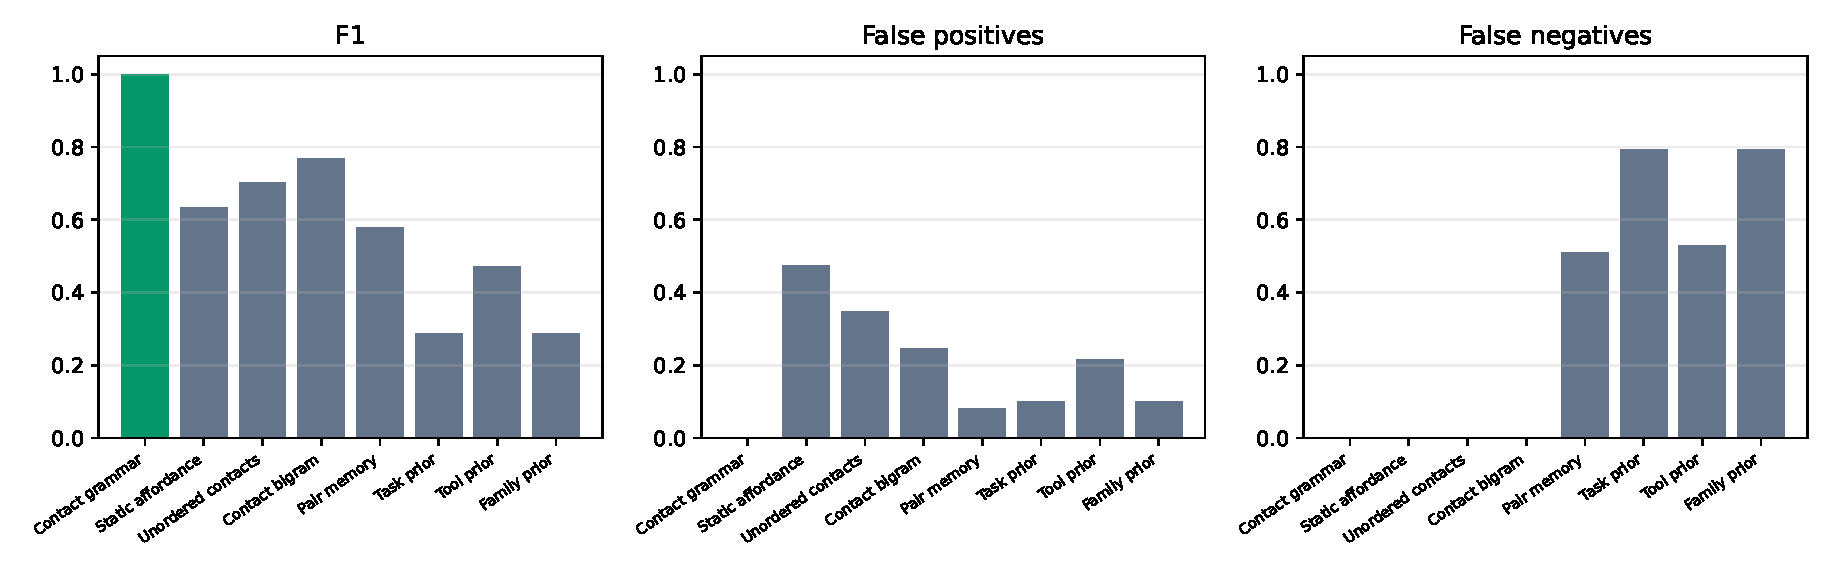
\includegraphics[width=\linewidth]{figures/full_scale_main_metrics.pdf}
\caption{Full-scale baseline metrics. The contact grammar removes false positives caused by ignoring role, side, support, and order.}
\label{fig:main}
\end{figure}

The result should not be read as a claim that the grammar is learned or physically complete. It says that, when the symbolic predicates are reliable and the production library matches the oracle, the ordered role representation separates valid and invalid traces that coarser representations conflate. The baselines are intentionally simple because the point is to isolate assumptions: if order and role are removed, false positives appear.

\section{Production Mutation Audit}

Table~\ref{tab:mutation} and Figure~\ref{fig:mutation} test falsifiability. Dropping the friction gate gives false-positive rate 0.105 and F1 0.876. Dropping the side gate gives false-positive rate 0.084 and F1 0.898. Dropping length or stiffness gates gives false-positive rate 0.062. Dropping the brace gate gives a smaller but still measurable false-positive rate 0.018. These are not arbitrary performance drops. Each mutation corresponds to a physical story: accepting a blocked-side contact, an unbraced pry, an insufficiently long tool, a too-compliant force tool, or a low-friction contact on a slippery surface.

\begin{table}[t]
\centering
\small
\caption{Production mutation audit. Removing individual gates creates interpretable false-positive signatures.}
\label{tab:mutation}
\begin{tabular}{lrrr}
\toprule
Mutation & F1 & FP rate & FN rate \\
\midrule
drop-side-gate & 0.898 & 0.084 & 0.000 \\
drop-brace-gate & 0.976 & 0.018 & 0.000 \\
drop-length-gate & 0.922 & 0.062 & 0.000 \\
drop-stiffness-gate & 0.922 & 0.062 & 0.000 \\
drop-fragility-gate & 0.986 & 0.011 & 0.000 \\
drop-friction-gate & 0.876 & 0.105 & 0.000 \\
\bottomrule
\end{tabular}

\end{table}

\begin{figure}[t]
\centering
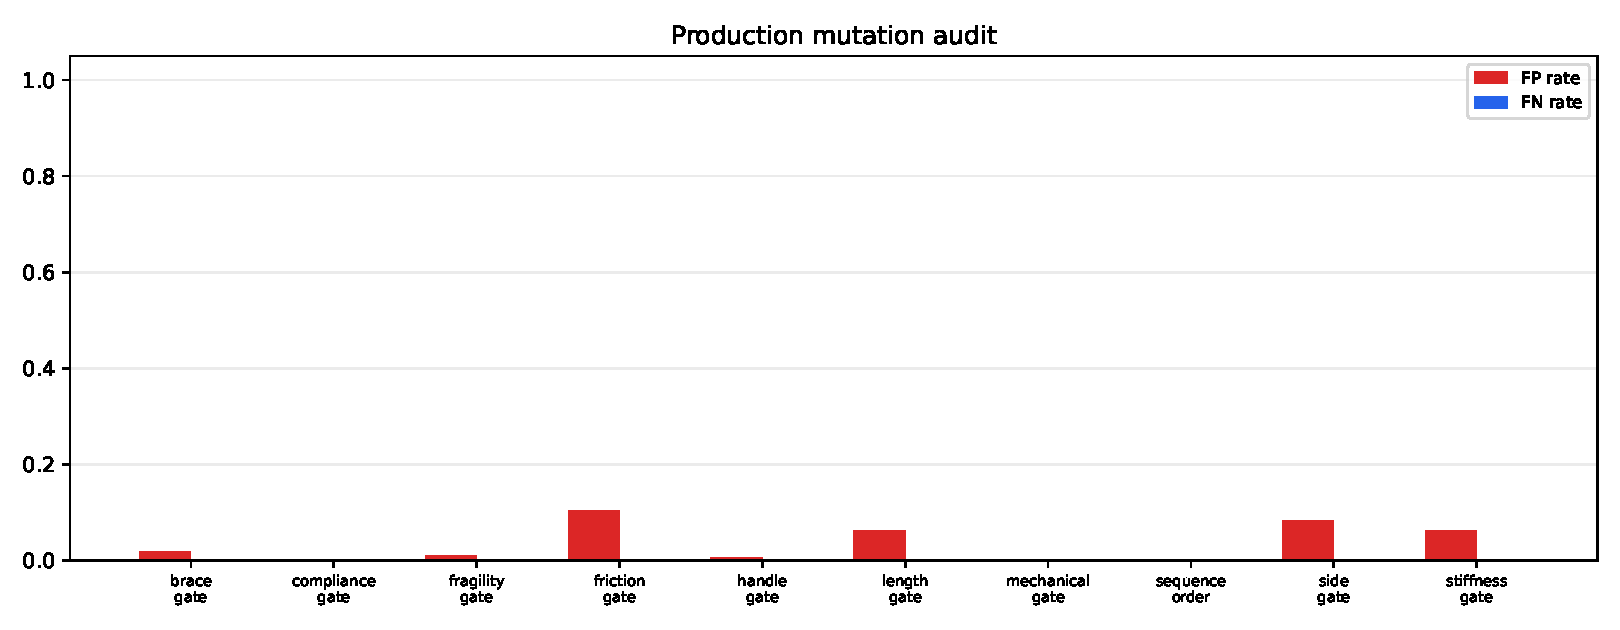
\includegraphics[width=\linewidth]{figures/full_scale_mutation_audit.pdf}
\caption{Mutation audit. Bars show false-positive and false-negative rates after individual precondition gates are removed.}
\label{fig:mutation}
\end{figure}

Some mutations have no effect in the sampled suite. Dropping the compliance or mechanical wedge gate yields no measurable change because other gates or required feature checks already rule out the sampled invalid cases. This is useful information: it shows which rules are redundant under the current generator and which gates carry independent falsification burden.

\section{Predicate Noise}

The clean grammar assumes reliable typed symbolic observations. Table~\ref{tab:noise} and Figure~\ref{fig:noise} stress that assumption. Under independent predicate noise, direct grammar F1 falls from 1.000 to 0.912 at 5\%, 0.861 at 10\%, 0.731 at 20\%, and 0.642 at 30\%. False positives rise from 0.000 to 0.079 at 30\%; false negatives rise more sharply because dropped or perturbed predicates make valid derivations look impossible.

\begin{table}[t]
\centering
\small
\caption{Independent predicate-noise stress. The probe fallback is an idealized symbolic audit, not a real perception model.}
\label{tab:noise}
\begin{tabular}{lrrrr}
\toprule
Noise & Direct F1 & Direct FP & Fallback F1 & Fallback probes \\
\midrule
0\% & 1.000 & 0.000 & 1.000 & 3.06 \\
5\% & 0.912 & 0.022 & 1.000 & 3.14 \\
10\% & 0.861 & 0.041 & 1.000 & 3.17 \\
20\% & 0.731 & 0.058 & 1.000 & 3.31 \\
30\% & 0.642 & 0.079 & 1.000 & 3.37 \\
\bottomrule
\end{tabular}

\end{table}

\begin{figure}[t]
\centering
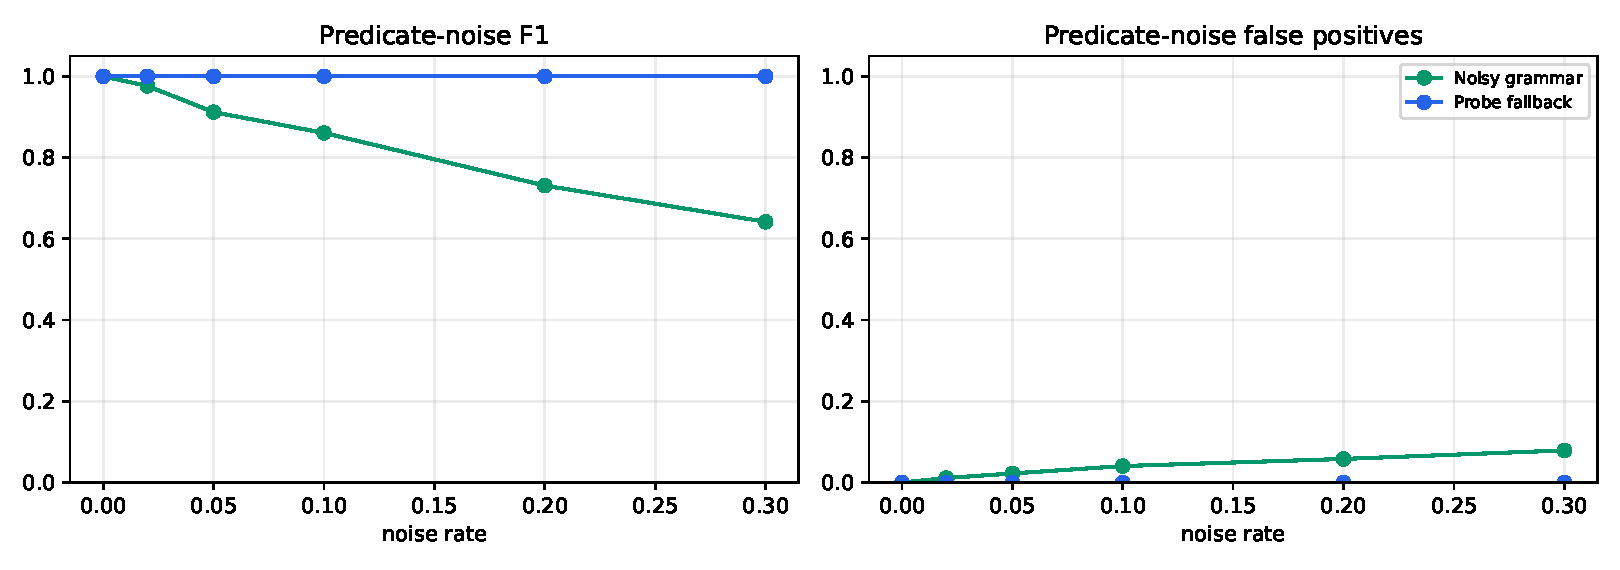
\includegraphics[width=\linewidth]{figures/full_scale_predicate_noise.pdf}
\caption{Predicate-noise stress. Direct grammar degrades as symbolic observations are corrupted; targeted probe fallback restores the symbolic oracle at a probe cost in this abstraction.}
\label{fig:noise}
\end{figure}

The targeted-probe fallback restores F1 1.000 in this simulator, but it is deliberately idealized. It probes rejected or suspicious derivations against the true symbolic state. Its mean probe count is 3.17 at 10\% noise and 3.37 at 30\% noise. The result is best understood as a boundary: the grammar representation is not robust to noisy perception by itself. It needs calibrated predicates, verification, or targeted probing.

\section{Granularity and Library Incompleteness}

Role granularity matters. The fine grammar has F1 1.000. Coarse side roles reduce F1 to 0.917 and create false-positive rate 0.065. Removing environment roles gives F1 0.974 and false-positive rate 0.020. Removing all roles gives the same F1 0.917 as coarse sides in this stress. Unordered derivation has no effect in the sampled suite because the current oracle's order-sensitive failures are mostly encoded through side and support gates; this is a limitation of the generator and a target for future expansion.

Library incompleteness fails mostly safely. Removing hook-pull productions gives F1 0.933 and false-negative rate 0.125, with false-positive rate 0.000. Removing wipe productions gives F1 0.959 and false-negative rate 0.080. Removing clamp, pry, lever, or separation productions produces smaller false-negative increases. This is the desired behavior for missing rules: the planner should reject valid traces it cannot derive rather than accept invalid traces as valid.

\begin{table}[t]
\centering
\small
\caption{Grammar-library incompleteness. Missing production families mainly create false negatives, which is safer than accepting invalid traces.}
\label{tab:library}
\begin{tabular}{lrrr}
\toprule
Missing family & F1 & FP rate & FN rate \\
\midrule
clamp & 0.984 & 0.000 & 0.031 \\
hook-pull & 0.933 & 0.000 & 0.125 \\
lever & 0.992 & 0.000 & 0.015 \\
pry & 0.985 & 0.000 & 0.029 \\
separate & 0.989 & 0.000 & 0.021 \\
wipe & 0.959 & 0.000 & 0.080 \\
\bottomrule
\end{tabular}

\end{table}

\begin{figure}[t]
\centering
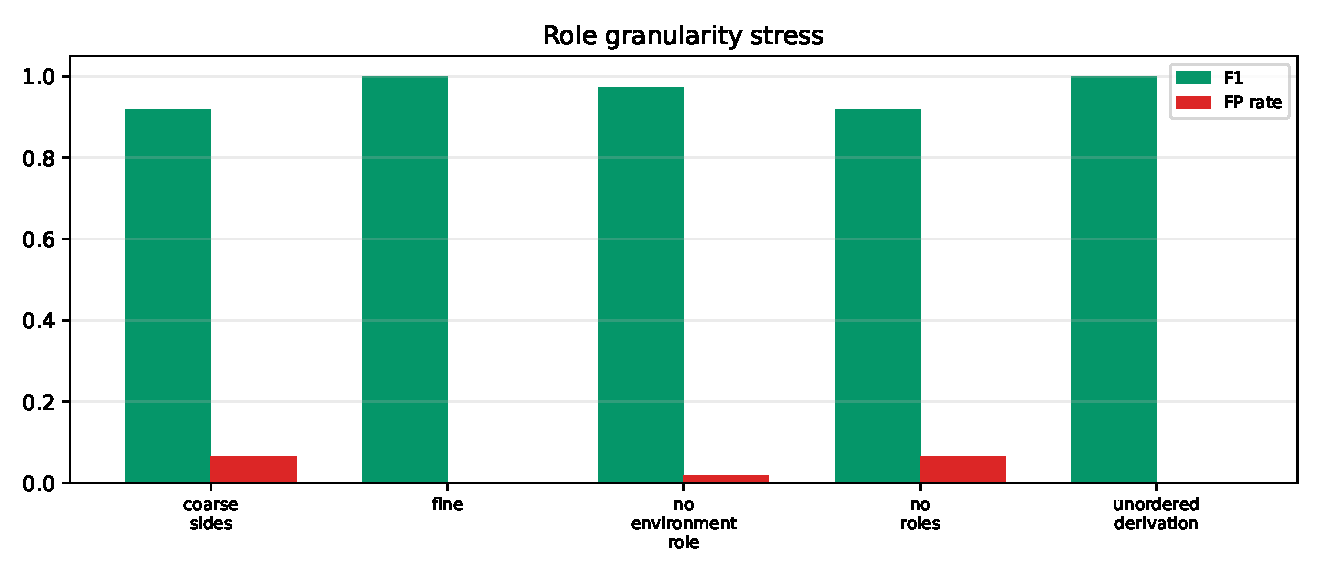
\includegraphics[width=0.86\linewidth]{figures/full_scale_granularity.pdf}
\caption{Role granularity stress. Coarsening sides or removing roles moves the grammar toward affordance-like false positives.}
\label{fig:granularity}
\end{figure}

\section{Counterexamples}

The counterexample suite constructs all-invalid slices where feature-only or unordered methods should fail. In blocked-side counterexamples, unordered contacts, static affordances, and contact bigrams have false-positive rate 1.000; the fine grammar has false-positive rate 0.000. The same pattern appears for missing braces and bad handle offsets. In fragile-force counterexamples, static affordance and unordered contacts accept the invalid traces, while the contact bigram and grammar reject them because they include a fragility or force gate. In slippery-surface counterexamples, static affordance, unordered contacts, and bigrams accept invalid traces when friction role is ignored; the grammar rejects them.

\begin{figure}[t]
\centering
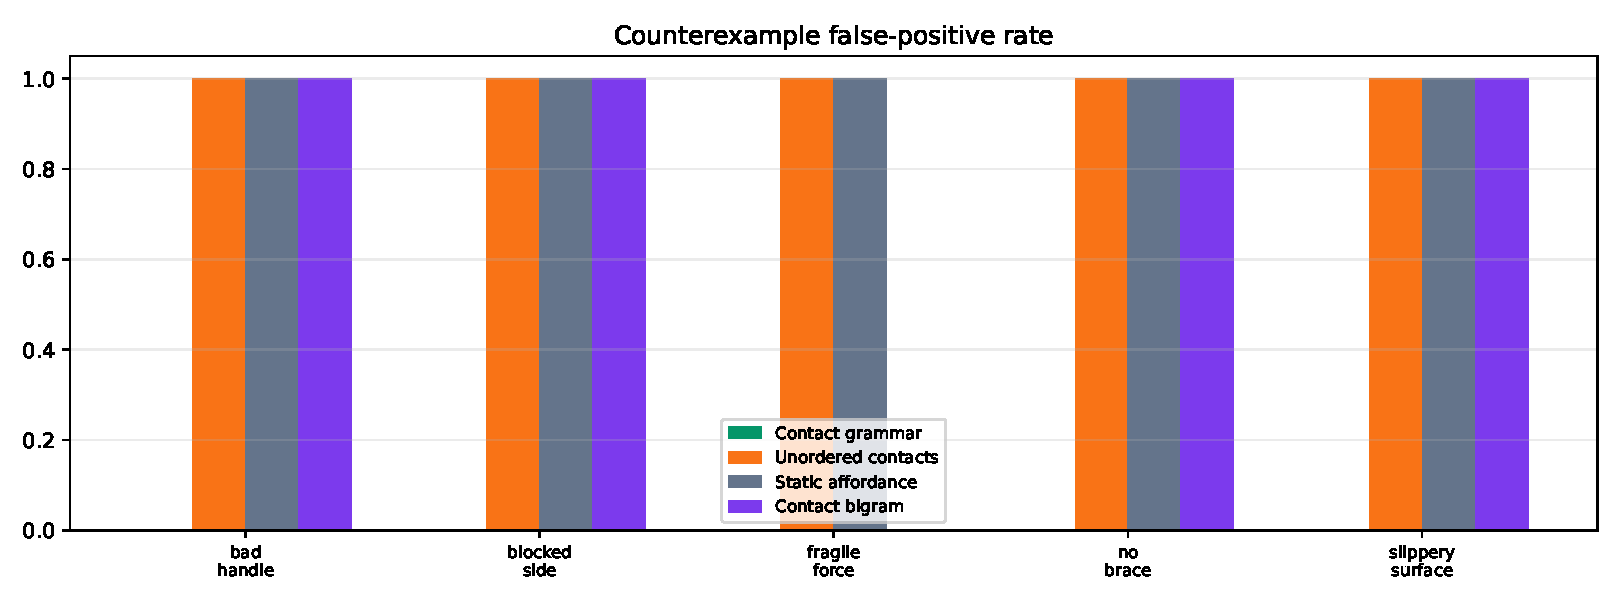
\includegraphics[width=\linewidth]{figures/full_scale_counterexamples.pdf}
\caption{Adversarial counterexamples. Feature and unordered-contact methods accept invalid traces that violate side, support, force, friction, or hand-tool role preconditions.}
\label{fig:counterexamples}
\end{figure}

These counterexamples are not meant to be a natural distribution. They are unit tests for the representation. A contact grammar should reject a tool that has the right feature in the wrong role; an affordance label often cannot express that distinction.

\section{Discussion}

\subsection{What the Grammar Adds}

\CG{} adds an explicit symbolic contact trace. Instead of saying that a tool affords pulling, it says that the hand grasps the handle, the hook seats behind or inside the target, side access is available, the tool has enough length, and the draw or lift production can consume that contact. The representation is compositional because productions can be reused across tasks. It is falsifiable because each precondition can be removed and tested.

\subsection{When It Is Appropriate}

The abstraction is appropriate when tool-use validity depends on contact roles that can be estimated or verified. It is less appropriate when contact dynamics are too continuous or high-dimensional to be summarized by symbolic roles, when perception cannot reliably estimate predicates, or when the production library is unknown. In those cases, the grammar may still serve as a hypothesis generator or explanation layer, but it should not be the sole planner.

\subsection{Why Static Affordances Are Not Enough}

Static affordances are useful for identifying possible actions, but they do not necessarily encode side, support, sequence, or force transmission. A hook may afford pulling only if it is seated behind or inside the target. A wedge may afford prying only with a brace. A soft pad may afford wiping but not tamping. The full-scale results quantify these distinctions: feature-only methods have high recall but high false-positive rates.

\subsection{Why Verification Still Matters}

The predicate-noise stress is the main warning. Direct grammar planning is exact only when symbolic observations are exact. At 20\% noise, F1 falls to 0.731 and false-negative rate rises sharply. A deployed robot would need tactile/vision estimators, calibrated uncertainty, and selected-production verification. The targeted-probe fallback in this paper is an idealized upper bound, not a solved perception system.

\section{Limitations}

The evidence is a finite symbolic world, not a real robot. The production library is hand-designed. The oracle uses the same symbolic vocabulary as the grammar, so the main result is a clean mechanism test rather than independent physical validation. Continuous contact stability, friction cones, slip, deformation, tool breakage, tactile sensing, and controller synthesis are coarse predicates. The perception-noise suite is synthetic; it does not replace real perception experiments. The cost analysis is secondary and illustrative. A stronger robotics claim would need learned or calibrated contact predicates, contact-rich control integration, and hardware or high-fidelity simulation.

\section{Reproducibility}

The legacy v2 experiment is reproduced with:
\begin{center}
\texttt{python experiments/contact\_grammar\_eval.py}
\end{center}
The full-scale final pass is reproduced with:
\begin{center}
\texttt{python experiments/full\_scale\_contact\_grammar.py}
\end{center}
The full-scale script writes streamed CSVs and summaries under \texttt{data/full\_scale/}, figures under \texttt{paper/figures/}, and the final summary in \texttt{docs/full\_scale\_results\_summary.md}. The run is deterministic under fixed seeds and uses standard Python plus Matplotlib.

\section{Ethics Statement}

The paper does not deploy robots. The intended safety benefit is to reject physically invalid tool-use traces before execution. A real deployment could still be unsafe if symbolic predicates are wrong, if the grammar omits an important contact mode, or if the continuous controller fails to realize a symbolic contact. Safety-critical use would require independent verification, force/torque limits, runtime monitoring, and human-approved recovery policies.

\section{Conclusion}

Tool use is not only object category plus action label. It is an ordered contact process over hand, tool, target, and environment roles. \CG{} makes that process explicit. In the expanded symbolic contact world, the fine grammar rejects invalid traces that static affordances, unordered contacts, and local contact models accept. The same experiments expose the boundary: if predicates are noisy or rules are missing, direct grammar planning needs fallback verification or abstention. The final claim is therefore precise: contact-role productions are a sharper representation and falsification language for robot tool use under reliable typed observations, not a complete robot tool-use system.

\bibliographystyle{iclr2026_conference}
\bibliography{references}

\appendix
\renewcommand{\thesection}{A\arabic{section}}
\renewcommand{\thesubsection}{A\arabic{section}.\arabic{subsection}}

\section{Production Library}

The simulator implements a compact production family rather than a separate handwritten rule for every task. Each task names a sequence, but productions share gates. A grip production establishes hand-tool role. Side-contact productions establish front, behind, under, inside, top, or side contact. Support productions establish environment brace. Force productions check stiffness, friction, compliance, fragility, and handle offset. Terminal productions consume the relevant contact state.

The rule library is deliberately interpretable. A failed \textsc{SeatHookBehind} production reports whether the hook feature is missing, the tool is too short, or the side is blocked. A failed \textsc{RotateAboutBrace} reports missing brace or missing wedge mechanics. A failed \textsc{WipeSurface} reports missing compliance or insufficient friction. This is useful for repair: the planner can request a different tool, change side approach, add a brace, or probe a predicate.

\section{Task Families}

The 15 task families cover different contact roles.
\begin{center}
\small
\begin{tabular}{lll}
\toprule
Family & Required contact story & Primary failure gates \\
\midrule
Hook pull & seat hook behind & side, length, hook feature \\
Sweep & lay flat edge front & side, friction, flat edge \\
Pry & insert wedge and brace & brace, wedge, stiffness \\
Press & align tip and press & length, stiffness, tip \\
Drag & thread hook inside & inside side, length, hook \\
Tamp & place flat end top & stiffness, fragility \\
Scrape & angle sharp edge & friction, stiffness, sharp edge \\
Scoop & slide bowl under & side, bowl, length \\
Lever & wedge under and lever & brace, handle offset, stiffness \\
Hook lift & seat hook inside & hook, stiffness, inside contact \\
Clamp & align jaw side & clamp jaw, friction, stiffness \\
Twist & seat torque handle & handle offset, friction, stiffness \\
Wipe & place soft pad & compliance, friction \\
Stir & insert long shaft & length, inside contact \\
Separate & insert thin lip and brace & thin lip, wedge, brace \\
\bottomrule
\end{tabular}
\end{center}

The task set is not intended to cover all real tool use. Its purpose is to create varied symbolic pressures on contact role, order, morphology, and environment support.

\section{Method Details}

\subsection{Static Affordance}

The static affordance baseline checks only whether the tool has the required functional features. For wiping, it also checks for soft-pad-like compliance. This baseline is high recall because it accepts many tools with the right feature. Its weakness is false positives: a feature can exist but be used from the wrong side, without a brace, or with unsafe force.

\subsection{Unordered Contacts}

The unordered-contact baseline checks required features and length but ignores side, brace, role order, friction, fragility, and handle offset. It represents a method that knows the necessary parts can touch but not how the contact story unfolds.

\subsection{Contact Bigram}

The contact-bigram baseline adds some local gates: feature, length, stiffness, and fragility. It improves over static affordance and unordered contacts, but it lacks the full hand-tool-target-environment role derivation. It is a useful intermediate because it shows that local contact checks help but do not replace role order.

\subsection{Flat Pair Memory and Priors}

Flat pair memory accepts task-tool signatures seen as valid in training. It has a lower false-positive rate than feature-only methods, but high false-negative rate on held-out valid compositions. Task, tool, and family priors expose how much can be recovered from empirical rates without contact structure.

\section{Noise Models}

The full-scale predicate-noise suite corrupts the observation passed to the grammar while scoring against the true oracle.
\begin{itemize}
    \item \textbf{Independent}: features, attributes, sides, brace, fragility, and slipperiness are corrupted independently.
    \item \textbf{Feature drop}: true tool features are omitted.
    \item \textbf{False feature}: spurious tool features are added.
    \item \textbf{Side-role swap}: blocked side and contact side observations are especially noisy.
    \item \textbf{Correlated sensor}: one sensor failure can corrupt many predicates in the same episode.
    \item \textbf{Morphology bias}: hook-related morphology is more likely to be missed.
\end{itemize}

Feature drops usually create false negatives because valid tools look incomplete. False features and side swaps create false positives because invalid traces appear to have the needed morphology or access. Correlated failures are important because real perception errors are rarely independent.

\section{Cost Interpretation}

The cost-sensitivity file recomputes total cost from behavior components: derivation steps, predicate checks, probes, invalid accepted traces, and valid rejected traces. The cost model is not central to the paper, but it prevents a universal-dominance claim. If invalid accepted plans are cheap and predicate probes are expensive, a coarse method may be cheaper despite worse symbolic validity. If invalid tool-use attempts are expensive, the fine grammar's low false-positive rate is valuable.

In real robot tool use, the costs would depend on hardware risk. A false-positive pry could break a tool or target. A false-negative wipe might merely ask for another tool. A missed brace in a lever task could be dangerous. The simulator does not calibrate these values; it only exposes which error type each representation tends to make.

\section{Additional Counterexample Details}

\subsection{Blocked Side}

The blocked-side case uses a tool with the right feature but blocks the side required by the task. Static affordance and unordered contacts accept the trace because the feature exists. The grammar rejects it through the side gate.

\subsection{Missing Brace}

The no-brace case uses a wedge-like tool for a pry or lever task but removes environment support. Methods that do not model environment role accept the trace. The grammar rejects it through the brace gate.

\subsection{Fragile Force}

The fragile-force case uses a stiff tool on a fragile target. Feature methods accept because the tool has the right end. The grammar rejects if stiffness exceeds the task's fragile limit.

\subsection{Slippery Surface}

The slippery-surface case uses the right edge but insufficient friction. The grammar rejects through the friction gate. Feature-only methods accept because they do not represent force transmission quality.

\subsection{Bad Handle Offset}

The bad-handle case uses a wedge/shaft tool for levering but with a poor hand-tool role. The grammar rejects through handle offset because the tool cannot transmit torque as required.

\section{Detailed Failure Taxonomy}

\subsection{False Positives}

False positives are physically invalid traces accepted by a representation. They are the most important safety error in this paper because they correspond to a robot attempting a tool-use action whose symbolic contact story is incomplete or wrong. The full-scale generator creates several false-positive families. A \emph{feature false positive} occurs when the tool has the required morphology but the task's contact side is blocked. A \emph{support false positive} occurs when a wedge or lever tool exists but the environmental brace required for force transmission is absent. A \emph{force false positive} occurs when a tool is too compliant, too rigid for a fragile target, or has insufficient friction. A \emph{role false positive} occurs when the hand-tool relation cannot transmit the needed torque or normal force.

Static affordances create many feature false positives because they only check required tool parts. Unordered contacts reduce some missing-feature errors but still accept side and support failures. Contact bigrams reduce some force errors but miss global role structure. The fine grammar rejects these because each production gate is tied to a particular physical role.

\subsection{False Negatives}

False negatives are valid traces rejected by a representation. They matter because a robot may miss a feasible solution. Flat pair memory has high false-negative rate because it rejects held-out task/tool compositions even when the tool has the right contact story. Library incompleteness creates false negatives when a production family is absent. Predicate noise also creates false negatives when true features are dropped or attributes are perturbed below a threshold.

False negatives are safer than false positives in the sense that the robot does not execute an invalid trace, but they can still be costly or unacceptable. A search system that rejects too many valid derivations may fail a task, ask for unnecessary human help, or choose a much worse tool. This is why the paper tracks both error types rather than reporting only F1.

\subsection{Abstention}

The full-scale fallback is best interpreted as an abstention-plus-probe layer. When the grammar is uncertain or rejects a derivation under noisy observations, the system can query targeted predicates. In the symbolic world this recovers the true state, so F1 returns to 1.000. In a real robot, probes would be tactile checks, visual re-observations, force tests, or short guarded motions. The simulator does not claim those probes are free or reliable; it only shows where they would be needed.

\section{Rule-by-Rule Interpretation}

\subsection{Side Gate}

The side gate says that a contact production requiring a specific target side cannot proceed if that side is blocked, unless the tool morphology can legitimately reach around or into the blocked region. Hooks, wedges, thin lips, and narrow tips can sometimes bypass blocked-side conditions; broad flat edges cannot. Dropping this gate creates false positives in blocked-side and sweeping counterexamples. This is the cleanest demonstration that a feature label is not enough: a flat edge exists, but it is on the wrong side of the task.

\subsection{Brace Gate}

The brace gate represents environment participation in the contact chain. Prying and levering are not only tool-target contacts. They require a third relation: the tool must brace against an environment or target rim so rotation creates useful force. Dropping the brace gate creates accepted pries without support. This is a role error rather than a morphology error. The wedge is present, but the force path is incomplete.

\subsection{Length Gate}

The length gate distinguishes tools that have the right feature but cannot reach the target relation. A hook that is too short cannot pull a distant ring. A narrow tip that is too short cannot press a recessed button. A wedge that cannot reach under a target cannot pry even if it has the right local geometry. Dropping length creates false positives that static affordances often make by default.

\subsection{Stiffness and Compliance Gates}

Stiffness and compliance gates encode force compatibility. Tamping, pressing, prying, scraping, and levering require enough stiffness. Wiping requires compliance. A soft brush can wipe but not pry; a steel wedge can pry but may damage fragile powder or soft material. These gates are coarse, but they force the representation to state which mechanical property is required.

\subsection{Friction Gate}

The friction gate is the largest mutation failure in the full-scale audit. Dropping it yields false-positive rate 0.105. This happens because scraping, sweeping, clamping, twisting, and separation require force transmission through a contact patch. A tool may have the right shape but slip under load. The symbolic friction gate is not a friction cone, but it marks that the contact relation must be verified at all.

\subsection{Handle Gate}

The handle gate is the hand-tool part of the role system. Tool use is not only tool-target contact. The robot must grasp in a way that transmits the required wrench. A long shaft with a bad handle offset may touch the target but fail to apply leverage. The handle gate catches this class of bad derivations.

\section{Expanded Suite Rationale}

\subsection{Why Five Profiles}

The five main profiles are designed to shift the source of invalidity. Baseline mixes all gates. Hard access increases blocked-side failures. Scarce support increases brace failures. Fragile targets increase force-limit failures. Morphology OOD stresses held-out signatures and memory baselines. This matters because a representation can look good on one profile while failing on another. For example, a method that checks side but not brace can survive hard access but fail scarce support.

The grammar is exact across these profiles because it mirrors the symbolic oracle. The baselines change differently. Static affordance degrades when more invalidity comes from side, support, or force gates. Flat memory degrades when morphology OOD increases the number of unseen valid task/tool signatures. Contact bigram is strongest when local gates suffice and weakest when global environment or hand-tool roles matter.

\subsection{Why Mutation Audits}

Mutation audits are included because high aggregate accuracy can hide nonessential rules. If removing a precondition never changes behavior, that precondition may be redundant under the current world distribution. If removing it creates a specific false-positive class, the rule has empirical bite. The mutation table therefore functions like an ablation map over the production library. The result is mixed in a useful way: side, friction, length, and stiffness gates matter strongly; compliance and mechanical gates are redundant in the sampled suite because other checks catch the same cases.

\subsection{Why Counterexamples}

Natural random episodes can under-sample rare but important physical errors. Counterexamples are controlled unit tests. They ask whether a representation rejects traces that are invalid for one known reason. The all-invalid slices make F1 less informative because there are no positives; false-positive rate is the intended metric. In blocked-side, no-brace, bad-handle, and slippery-surface slices, the grammar's false-positive rate is 0.000 while coarser methods often reach 1.000. These tests explain the aggregate false-positive rates in a more concrete way.

\subsection{Why Library Incompleteness}

No hand-written grammar is complete. The library-incompleteness suite asks what happens when a family of productions is missing. The desired behavior is conservative failure: reject derivations that require missing productions. That creates false negatives but not false positives. This is what the suite shows. The implication for deployment is that missing rules should be visible as capability gaps, not hidden as unsafe accepted plans.

\section{Predicate-Noise Semantics}

\subsection{Feature Drops}

Feature drops simulate perception missing a tool part. A hook may not be recognized, a thin lip may be occluded, or a soft pad may be misclassified. This usually creates false negatives: the grammar rejects a trace that would be valid if the feature were observed. Feature drops are therefore mostly a completeness and usability issue.

\subsection{False Features}

False features simulate hallucinated or overgeneralized morphology. A rounded edge may be mistaken for a wedge, or a soft pad may be mistaken for high-friction contact. This creates false positives because the grammar believes a production precondition is satisfied when it is not. False features are more dangerous than feature drops when they enable forceful tool actions.

\subsection{Side-Role Swaps}

Side-role swaps corrupt the target-side relation. This is especially damaging for hooks, wedges, and brushes because validity often depends on whether contact occurs in front, behind, under, inside, or on top of the target. A side-role swap can turn an invalid blocked-side trace into an apparently valid one or turn a valid trace into a false negative.

\subsection{Correlated Sensor Failure}

The correlated-sensor scenario models a bad observation event that corrupts many predicates at once. Real perception errors are often correlated: lighting, occlusion, calibration, or viewpoint can affect features, sides, and attributes together. Independent noise is easier for a planner to tolerate. Correlated noise can move an entire derivation into the wrong symbolic state.

\subsection{Morphology Bias}

Morphology bias increases errors for hook-related families. This tests whether the conclusion depends on uniformly reliable features. A real robot might be better at detecting flat edges than hook seating, or better at estimating length than compliance. The grammar can only be as good as the predicate channels needed by the current task family.

\section{Data Generation Details}

\subsection{Tools}

Tools are generated from templates and random feature combinations. Templates include hook rods, rubber hooks, steel spatulas, wedge bars, soft brushes, tampers, scoops, clamps, and torque drivers. Random tools combine one to four morphology predicates. Attributes are sampled from bounded integer ranges. Feature-specific adjustments make the world less arbitrary: long-shaft tools are longer, soft-pad tools are more compliant and less stiff, wedge and sharp-edge tools are stiffer, and high-friction tools have higher friction.

\subsection{Episodes}

Each episode samples a task and tool. With higher probability, the generator chooses a tool containing the task's required features, ensuring enough positive cases. It then samples blocked side, brace availability, target fragility, and target slipperiness. The training split provides seen task/tool signatures for memory and prior baselines; the test split evaluates generalization.

\subsection{Oracle}

The oracle checks a conjunction of gates. This makes the experiment transparent. The oracle is not independent of the grammar; both use the same symbolic vocabulary. That is a limitation for physical claims, but it is appropriate for the representational mechanism test. The point is to ask which abstractions preserve the symbolic validity function and which collapse it.

\subsection{Metrics}

Metrics are computed over oracle labels and method predictions. Precision and recall are included through F1, but false-positive and false-negative rates are reported directly because they have different robotics meanings. Mean steps and predicate checks are recorded for cost analysis. Mean probes are recorded for fallback methods.

\section{Cost-Regime Notes}

\subsection{Accepted Invalid Trace Cost}

An accepted invalid trace can be benign or dangerous depending on the task. A failed wipe may leave a surface dirty. A failed pry may damage the target. A failed twist may strip a knob. The cost-sensitivity file lets this penalty vary. When accepted invalid traces are costly, the grammar's low false-positive rate dominates.

\subsection{Rejected Valid Trace Cost}

A rejected valid trace is a missed opportunity. It can force the robot to choose another tool, ask for help, or fail the task. Memory baselines and incomplete grammars often create this cost. In a setting with many alternative tools, false negatives may be tolerable. In a constrained setting, they may be severe.

\subsection{Probe Cost}

Probe cost is the price of resolving symbolic uncertainty. The fallback method probes several predicates even in clean settings because it audits rejected or suspicious derivations. This is intentionally conservative. A real system would use confidence thresholds to probe only uncertain predicates, but then the result would depend on calibrated perception. The paper keeps the fallback idealized to show the upper bound.

\section{Relationship to Continuous Control}

\CG{} does not synthesize torques or trajectories. It says which contact relations must be achieved. A continuous controller could be called for each production. For \textsc{SeatHookBehind}, the controller would move the hook around the target and verify seating. For \textsc{BraceOnRim}, it would establish support. For \textsc{RotateAboutBrace}, it would apply torque under force limits. If the controller cannot realize a predicate, it returns the failed production precondition.

This interface is useful because it turns low-level failure into symbolic repair information. Instead of returning ``trajectory failed,'' the controller can return ``brace contact missing'' or ``tool slipped at friction gate.'' The grammar can then choose another derivation, another tool, or a targeted probe. The present paper does not implement that controller loop, but the production vocabulary is designed for it.

\section{Learning and Calibration Path}

The production library is hand-designed in this work. A natural next step is to learn precondition thresholds or production applicability from robot experience. For example, the stiffness threshold for pressing could be learned from force outcomes, and the side-access gate for hooks could be learned from successful seating attempts. The grammar would provide structure: learning estimates the parameters of named productions rather than discovering an unstructured policy.

Calibration also matters for perception. A vision model might output confidence over tool features and contact sides. A tactile model might estimate whether a hook is seated or a brace is loaded. These confidences could drive the probe fallback. High-confidence predicates pass directly; uncertain predicates trigger active checks. The full-scale noise suite identifies which predicate families most need calibration.

\section{Additional Limitations}

The generator is symbolic and hand-crafted. Because the grammar matches the oracle vocabulary, the clean F1 1.000 result should not be interpreted as independent validation. The result is valuable because coarser baselines fail under the same oracle. Still, a real-world paper would need independent labels from physical trials.

The current order sensitivity is underdeveloped. The unordered-derivation granularity variant does not fail in the sampled suite because many order requirements are encoded as side or support gates. A stronger future simulator should explicitly represent transient contacts and delete effects so that wrong order creates additional false positives.

The fallback is too strong. It probes true symbolic state directly. This is useful as an upper bound but not a deployed method. Real probes can fail, cost time, or perturb the scene. Future work should model probe reliability and choose probes adaptively.

The task library is broader than the v2 paper but still small relative to real tool use. Cutting, fastening, scooping deformables, pouring, scraping with wear, and multi-tool sequences are not represented. The grammar idea should extend, but the current evidence does not prove that it does.

\section{Positive Findings}

The most important positive finding is not only that the grammar has high F1. It is that the grammar's advantage appears exactly where the hypothesis predicts: false positives caused by missing role, side, support, friction, or hand-tool relations. Static affordance and unordered contact baselines are high recall but unsafe in many invalid cases. Pair memory avoids some false positives but fails on valid held-out compositions. The grammar combines compositional reuse with explicit physical gates.

The second positive finding is that mutations are diagnostic. Removing gates creates interpretable failure signatures. This is useful scientifically because rules can be tested one by one. It is also useful for engineering because a failed deployment can ask which production precondition was wrong or missing.

The third positive finding is conservative library incompleteness. Missing production families mainly create false negatives. That is a safer default than accepting invalid traces, and it means a grammar can be extended incrementally as new tool-use families are added.

\section{Negative Findings}

The strongest negative finding is predicate noise. Direct grammar planning depends heavily on reliable symbolic observations. At 30\% independent noise, F1 falls to 0.642. This is not a small degradation. It means the grammar should not be deployed without perception calibration or verification.

The second negative finding is that some gates are redundant in the current generator. Dropping compliance, sequence-order, or mechanical gates has little or no measured effect. That does not mean these gates are unimportant in real tool use; it means the current suite does not stress them enough. The final claim therefore avoids saying every rule is empirically necessary.

The third negative finding is symbolic scope. The grammar can say that friction is required, but it does not compute a friction cone. It can say that a brace is needed, but it does not synthesize stable bracing contact. The representation is a planning abstraction, not a physics solver.

\section{Per-Profile Result Interpretation}

\subsection{Baseline}

The baseline profile mixes blocked sides, missing braces, fragile targets, and slippery contacts. It is the main summary because no single gate dominates. Static affordances reach F1 0.633 with false-positive rate 0.473; unordered contacts reach F1 0.702 with false-positive rate 0.347; contact bigrams reach F1 0.769 with false-positive rate 0.246. This ordering is meaningful. Each baseline adds some structure, and each added structure removes some invalid traces. But none of them has the full contact-role derivation, so false positives remain common.

\subsection{Hard Access}

The hard-access profile increases the probability that the task's required contact side is blocked. Static affordance falls to F1 0.581 with false-positive rate 0.515. Unordered contacts fall to F1 0.638 with false-positive rate 0.406. Contact bigrams fall to F1 0.715 with false-positive rate 0.284. This is exactly the profile where side role matters most. A feature can exist, and a local contact can look plausible, while the required target side is unavailable.

\subsection{Scarce Support}

The scarce-support profile increases failures for brace-required tasks. Static affordance has false-positive rate 0.471, unordered contacts 0.370, and contact bigrams 0.277. The grammar remains exact because brace is an explicit environment role. This profile highlights that tool use can involve more than hand, tool, and target. Environment support can be a necessary participant in the derivation.

\subsection{Fragile Targets}

The fragile-target profile increases the importance of force gates. Static affordance has F1 0.626 and false-positive rate 0.475. Contact bigram remains around F1 0.770 because it includes local fragility and stiffness checks. This is a case where a simpler local model captures much of the relevant structure. The grammar still has the advantage of combining force gates with side, brace, and hand-tool roles, but the profile shows that not every task needs the full grammar.

\subsection{Morphology OOD}

The morphology-OOD profile increases the number of tools and reduces the train fraction. Flat pair memory has F1 0.575 and false-negative rate 0.517. Its false-positive rate is low, but it rejects many valid held-out compositions. The grammar stays exact because productions apply compositionally to new tool signatures. This is the clearest generalization result: production structure is reusable where pair memory is not.

\section{Detailed Case Studies}

\subsection{Hook Pull}

A valid hook-pull derivation begins with a hand-tool grasp, then seats a hook behind or inside the target, then draws along the contact axis. A static affordance method sees only that the tool has a hook. An unordered contact method sees that hook and target can touch. The grammar asks whether the hook is seated on the correct side and whether the shaft is long enough. If the target's behind side is blocked and the hook cannot reach around it, \textsc{SeatHookBehind} fails before the draw production is considered.

\subsection{Pry}

A pry is a three-body contact story. The wedge must enter under the target, the tool must brace on a rim or environment support, and rotation must occur about the brace. A wedge feature alone is not a pry. The no-brace counterexample demonstrates this: static affordance, unordered contacts, and contact bigrams accept many wedge traces without environment support, while the grammar rejects them through \textsc{BraceOnRim}.

\subsection{Wipe}

Wiping needs compliance and friction more than stiffness. A hard flat edge may touch the surface but fail to wipe safely. A soft pad may wipe but fail to scrape. The grammar represents this by assigning different gates to wipe and scrape productions. This is why contact grammar should not be reduced to a single affordance label such as ``flat surface contact.'' The same geometry can play different roles under different force and compliance requirements.

\subsection{Lever}

Levering requires wedge insertion, length, handle offset, stiffness, and brace. The bad-handle counterexample shows that even a good wedge and long shaft are insufficient if the hand-tool role cannot transmit torque. This is a subtle failure for object-centric representations. The relevant contact is partly between the robot hand and the tool, not only between the tool and target.

\subsection{Twist}

Twisting a knob requires high friction and a torque handle. A tool with a long shaft but poor friction may be geometrically present but slip. The friction gate captures the role of tangential force transmission. The simulator's friction attribute is coarse, but the symbolic distinction matters: contact without traction is not the same as contact that can transmit torque.

\section{Extended Formal Counterexamples}

\subsection{Same Feature, Different Side}

Let a task require a front sweep and let the target's front side be blocked. Let a tool have a flat edge and sufficient length. A static affordance classifier accepts because the flat edge exists. An unordered contact model accepts because a tool-target contact label exists. A contact grammar rejects because the production requiring \texttt{tool:target\_front} cannot be applied. This proves that feature existence is insufficient for side-sensitive tasks.

\subsection{Same Contacts, Different Support}

Let a pry task require wedge-under and brace contacts. Consider two traces with the same tool-target wedge contact. In the first, an environment brace is established before rotation. In the second, no brace exists. An unordered tool-target representation cannot distinguish them if it does not include environment role. The grammar distinguishes them because \textsc{RotateAboutBrace} consumes a brace predicate.

\subsection{Same Tool, Different Target Fragility}

Let the same stiff flat-end tool be used for tamping two targets. One target is robust; one is fragile. Static tool affordance is identical in both cases. The grammar includes a task-target fragility gate and rejects the fragile case. This counterexample shows that tool-use validity is not only a property of the tool. It depends on the target and force context.

\subsection{Same Target, Different Hand-Tool Role}

Let a wedge tool be long enough and stiff enough for levering, but the robot grasps it at a poor handle offset. The tool-target relation is plausible, but the hand-tool relation cannot transmit the required torque. A grammar with hand-tool role rejects. A target-only contact representation accepts. This is why the representation names hand, tool, target, and environment explicitly.

\section{Hardware Validation Protocol}

\subsection{Minimal Robot Study}

A minimal hardware study would use a robot arm, a small tool rack, and a set of instrumented tabletop tasks: hook pull, pry, sweep, press, wipe, and twist. Each tool would have measured morphology and rough attribute estimates. Each task would have controlled side access, brace availability, target fragility, and surface friction. The robot would first plan with the grammar, then execute guarded controllers for each production.

The primary outcome would not be only task success. It would be whether the grammar rejects invalid traces before execution, whether selected productions fail for the predicted reason, and whether failure reports support repair. For example, when brace is removed, the system should reject prying or report brace failure. When side access is blocked, it should reject hook seating rather than attempting a pull.

\subsection{Perception Study}

A second study would calibrate symbolic predicates. Vision would estimate tool features, target side access, and morphology. Tactile or force sensing would verify seating, brace load, slip, and contact normal. The predicate-noise suite in this paper suggests which channels need attention: side roles, friction, and feature drops have strong effects. The study should report predicate calibration curves, not only final task success.

\subsection{Controller Integration}

A controller integration would map productions to guarded skills. \textsc{GraspHandle} would be a grasp controller. \textsc{SeatHookBehind} would be a guarded insertion or hooking controller. \textsc{BraceOnRim} would establish support under force limits. \textsc{RotateAboutBrace} would apply torque while monitoring slip and load. The grammar would supply the sequence and failure semantics; the controller would supply continuous realization.

\subsection{Benchmark Metrics}

Hardware metrics should include accepted invalid plan rate, rejected valid plan rate, task success, number of probes, number of production failures, repair success after failure, contact-estimator calibration, and execution safety events. These metrics mirror the symbolic paper but are grounded in robot data. A strong benchmark would include adversarial blocked-side, missing-brace, and slippery-surface cases.

\section{Comparison to Alternative Abstractions}

\subsection{Affordance Map}

An affordance map can say where a tool may be used, but it often does not encode derivation history. It may mark a hook region as useful for pulling without saying whether the hook is behind the target. A contact grammar can use affordance outputs as candidate predicates, but it then requires ordered role satisfaction.

\subsection{Contact Mode Sequence}

A contact mode sequence can be very expressive, especially in contact-rich planning. The grammar differs by making roles and falsification gates explicit at a symbolic level. It is less detailed than a continuous contact mode planner but easier to audit and compose over tool families. The two should be combined: grammar for symbolic trace hypotheses, continuous mode planning for feasibility.

\subsection{Language Plan}

A language plan can say ``use the wedge to pry the lid.'' The grammar expands that instruction into required contact roles: grasp wedge, insert under lid, establish brace, rotate. This expansion is where many physical failures become visible. A language model may choose a plausible tool, but the grammar checks the contact story.

\subsection{End-to-End Policy}

An end-to-end policy might learn tool use directly from demonstrations. Such a policy may succeed in-distribution but provide weak failure explanations. A grammar can serve as a structured prior or diagnostic layer. It can also help specify counterfactual tests: remove side access, remove brace, change target fragility, or swap tool compliance.

\section{Stress-Test Catalogue and Diagnostic Consequences}

\subsection{Blocked-Side Catalogue}

The blocked-side catalogue is the cleanest demonstration that tool use is not only a relation between a tool feature and a target class. A hook, wedge, scraper, or pad can exist, yet be unusable because the side required by the production is unavailable. The hard-access profile makes this failure common. Static affordances accept many such episodes because the feature predicate survives. Unordered contacts accept many of them because some contact between the tool and target can still be named. Contact bigrams reduce the error by encoding more local context, but they still miss global derivation constraints. The grammar rejects the trace because the relevant side production cannot fire.

The diagnostic value is high. A planner can say ``the hook cannot seat behind the target'' rather than simply ``pull failed.'' This is a different recovery problem. The robot might change viewpoint, move clutter, choose a longer hook, approach from another side, or abandon the task. These are all distinct from choosing another object with the same affordance label. The catalogue therefore tests not only classification accuracy but the usefulness of the failure language.

\subsection{No-Brace Catalogue}

The no-brace catalogue targets tasks where the environment is an active participant. Pry, lever, separate, and clamp-like actions often need a support or reaction contact. If the representation contains only tool-target contact, it can approve a wedge insertion even when no stable support exists for rotation or force closure. This is why the no-brace counterexample is severe: several baselines see the right tool and the right target contact, but they do not require the environment role.

The grammar treats brace as a consumed precondition for later force productions. A missing brace does not appear as a vague low-confidence decision. It appears as a falsified production. In a hardware system this matters because applying torque without support is not merely inefficient; it can damage the target, slip, or push the object away. A production failure can trigger an explicit repair: search for a rim, add a fixture, reposition the target, or choose a tool that can perform the task through a different contact sequence.

\subsection{Contact-Valid but Action-Invalid Catalogue}

Some invalid traces contain perfectly valid local contacts. A compliant pad can touch a surface but fail to scrape. A stiff scraper can touch a fragile target but be unsafe. A long rod can reach the target but fail to twist because friction is too low. These are contact-valid but action-invalid cases. They are important because a visual contact classifier can look successful even though the intended force transmission is impossible or unsafe.

The mutation audit is useful here. Dropping the friction gate produces F1 0.876 and false-positive rate 0.105. Dropping side, length, or stiffness gates produces smaller but still measurable losses. The numbers show that the gates are not decorative. They represent different physical assumptions. The paper's result is stronger when these assumptions are exposed individually: a reviewer can see which predicates matter, which sampled gates are currently redundant, and where future benchmarks should be made harder.

\subsection{Morphology-OOD Catalogue}

The morphology-OOD profile asks whether a method can reuse structure across tools. Flat pair memory is conservative: it avoids many false positives but rejects many valid held-out compositions, with false-negative rate 0.517. This is the failure mode expected from memorizing observed task-tool pairs. It is not enough to know that a particular training hook worked for a particular pull. A new hook with the same relevant production predicates should be considered.

The grammar handles this profile because productions are parameterized by roles and gates rather than instance IDs. A new tool can be accepted if it has the necessary hook, length, stiffness, handle, or compliance predicates. This is the positive generalization finding that motivates the representation. It does not prove sim-to-real transfer, but it does show that compositional symbolic structure gives a path to accepting novel tools without memorizing every pair.

\subsection{Missing-Library Catalogue}

The library-incompleteness suite is deliberately unfavorable to the grammar. When a task family is removed from the production library, valid episodes become false negatives. Missing hook-pull gives F1 0.933 and false-negative rate 0.125; missing wipe gives F1 0.959 and false-negative rate 0.080. False positives remain at zero in these slices because the model abstains rather than hallucinating a production.

This is the right failure shape for a safety-facing symbolic layer. A missing rule should cause rejection, not permission. The cost is coverage. The practical consequence is that a deployed system needs library discovery, learning, or human authoring. The experiment therefore avoids overselling the grammar: compositionality helps only inside the support of the production language. Outside that support, the system must ask for a new rule or route to another planner.

\section{Operational Reading of the Ablations}

\subsection{Why False Positives Dominate the Argument}

The paper reports accuracy, F1, false-positive rate, and false-negative rate, but the most safety-relevant number is often false-positive rate. A false negative rejects a valid plan and may cost time. A false positive approves an invalid contact trace and can damage the scene or robot. Under the baseline profile, static affordance has false-positive rate 0.473, unordered contacts 0.347, and contact bigrams 0.246. The grammar has zero false positives under reliable typed predicates.

The result should be read as a pruning result, not as a claim that symbolic grammar alone executes manipulation. The grammar removes physically inconsistent contact stories before continuous control. It reduces the number of dangerous traces that reach controllers. If the continuous controller is weak, execution can still fail. If perception is wrong, the grammar can still be fooled. Those are deployment problems, but they do not erase the representational finding.

\subsection{Why Fallback Probing Is Not a Free Lunch}

The predicate-noise suite includes a direct noisy grammar and a probe-fallback grammar. The direct grammar degrades to F1 0.861 at 10 percent independent predicate noise and 0.642 at 30 percent. The fallback grammar remains at F1 1.000 in this symbolic experiment because uncertain predicates can be queried against the clean latent state. That fallback is intentionally idealized. It should be interpreted as an upper bound on what targeted verification could provide, not as a deployed perception result.

The useful message is that a grammar localizes verification effort. Instead of validating every possible image feature, the robot can ask about predicates that matter to the selected derivation: Is the side blocked? Is the hook seated? Is there brace load? Is slip occurring? The mean probe count stays close to three in the synthetic suite because the production trace names a small number of critical predicates. A real system may need more probes, but it still benefits from knowing what to probe.

\subsection{Why Granularity Must Be Task-Dependent}

The granularity suite warns against a single fixed abstraction level. Removing side roles hurts because side access is task-critical. Removing the environment role hurts because brace can be necessary. By contrast, the unordered-derivation variant is not stressed hard enough in the present sampled suite and stays at F1 1.000. This is a useful negative result: not every coarsening fails under every task distribution.

The implication is that grammar design should be driven by failure modes. A household drawer-opening benchmark may stress side and handle roles. A cutting benchmark may stress stiffness, sharpness, and force limits. A cleaning benchmark may stress compliance, friction, and surface damage. The representation should name the contacts whose absence changes validity. The experiments here identify several such contacts, but they do not claim that this is a universal final vocabulary.

\section{Reviewer Audit Trail}

\subsection{What Would Falsify the Thesis}

The thesis would be weakened if a simpler representation matched the grammar across blocked-side, no-brace, fragile-target, slippery-surface, and morphology-OOD profiles while remaining equally interpretable. It would also be weakened if removing individual gates did not change behavior, because that would imply the production vocabulary is ornamental. The current experiments do not show that: static, unordered, bigram, prior, and memory baselines fail in different predictable ways, and several rule deletions produce measurable false positives.

The thesis would also be weakened if predicate noise made the grammar unrecoverable. The direct noisy results show degradation, but the fallback suite shows that targeted verification can in principle recover decisions when probes are available. A hardware paper must replace that idealized fallback with measured perception and touch. Until then, the claim remains a representation and simulation claim.

\subsection{What the Paper Does Not Claim}

The paper does not claim to learn the grammar from demonstration, solve continuous contact mechanics, replace contact planners, or prove real-world success. It does not claim that the production library is complete. It does not claim that all tool-use tasks reduce to the 15 families in the simulator. These limits are not cosmetic; they define the boundary between this paper and a future robot system.

The paper does claim that contact-role productions expose validity distinctions that common coarser abstractions erase. It claims that those distinctions matter in large symbolic stress tests. It claims that failure reports become more actionable when they identify a missing side, brace, length, friction, compliance, handle, or fragility predicate. It claims that a robot tool-use planner should represent an ordered contact story, not only a tool category or action verb.

\subsection{How the Final Version Should Be Read}

The final version should be read as a mechanism paper. The mechanism is not a neural architecture or a controller. It is a representation: a typed derivation over hand, tool, target, and environment contact roles. The positive finding is that this representation sharply reduces invalid acceptances under reliable predicates and generalizes compositionally across tool morphology. The negative finding is that predicates, rule coverage, and continuous execution remain hard. The value of the paper is that both sides are made explicit enough to test.

\section{Reviewer-Facing Boundaries}

A reviewer might say the grammar is just a symbolic planner. The response is that the symbolic vocabulary is the contribution: productions are organized around hand-tool-target-environment contact roles and falsifiable gates. Generic symbolic planning does not specify this contact-role hypothesis class.

A reviewer might say contact-rich planners already model contact. The response is that \CG{} is above continuous planning. It does not solve friction cones or contact-implicit control; it provides an interpretable role trace that can call those solvers with a better symbolic hypothesis.

A reviewer might say the result is tautological because the oracle and grammar share a symbolic vocabulary. This is partly true and explicitly scoped. The experiment is a mechanism test: if contact role and order are the right symbolic variables, coarser representations fail in predictable ways. Hardware validation is future work.

A reviewer might say perception noise breaks the method. The response is yes: direct grammar degrades under predicate noise. The paper quantifies this and treats targeted probes or verification as required for deployment.

\section{Deployment Sketch}

A deployed system would need to learn or engineer the production library, estimate predicates from vision and touch, and verify selected productions before forceful execution. A practical loop would:
\begin{enumerate}
    \item parse a task into a required terminal contact role;
    \item enumerate derivations from available tools and target/environment predicates;
    \item reject derivations whose preconditions fail;
    \item call perception or tactile probes for uncertain predicates;
    \item pass the selected derivation to a continuous controller;
    \item monitor whether each contact predicate is realized;
    \item if a production fails, report the falsified precondition and replan.
\end{enumerate}

The grammar is useful because the failure report is structured. ``No environment brace'' suggests adding support. ``Blocked side'' suggests a different approach. ``Too compliant'' suggests a stiffer tool. ``Bad handle offset'' suggests a different grasp or tool.

\section{Full-Scale Artifact Map}

\begin{center}
\small
\begin{tabular}{ll}
\toprule
Artifact & Purpose \\
\midrule
\texttt{main\_scaling\_trials.csv} & Per-episode rows for five operating profiles. \\
\texttt{main\_scaling\_summary.csv} & Aggregated method metrics by profile. \\
\texttt{mutation\_trials.csv} & Rule-gate mutation episodes. \\
\texttt{predicate\_noise\_trials.csv} & Direct and fallback grammar under noisy observations. \\
\texttt{granularity\_trials.csv} & Coarse side, no role, and unordered derivation variants. \\
\texttt{library\_incompleteness\_trials.csv} & Missing production-family stress. \\
\texttt{counterexample\_trials.csv} & Adversarial all-invalid unit tests. \\
\texttt{cost\_sensitivity\_summary.csv} & Recomputed cost grid. \\
\bottomrule
\end{tabular}
\end{center}

\section{Final Reproduction Checklist}

To regenerate the final evidence:
\begin{enumerate}
    \item run \texttt{python experiments/full\_scale\_contact\_grammar.py};
    \item confirm \texttt{data/full\_scale/progress.json} has stage \texttt{complete};
    \item build from \texttt{paper/} with \texttt{pdflatex}, \texttt{bibtex}, and two more \texttt{pdflatex} passes;
    \item confirm the PDF includes the full-scale figures and generated tables;
    \item confirm no obsolete process banner appears in the PDF text.
\end{enumerate}

\end{document}
